\chapter{Implementation and Results}
\label{cha:results}

In this chapter, we detail the implementation of various models and methods from both supervised and unsupervised learning to predict health metrics. We focus on their application, performance, and optimization. The analysis covers the used algorithms, the reasons for their selection and the achieved results. We want to highlight their predictive accuracy and reliability for health data. Additionally we want to predict a wide variety of features in this chapter, for example whether the test subject is sick or healthy.

\section{Supervised Learning Models}

In this section, we aim to evaluate the performance of supervised learning models on our dataset. The goal is to determine how well these models can predict health metrics based on the collected data before attempting to uncover correlations in relation to the 6MWT. We first prepared the dataset by cleaning and transforming the data, as previously described.

\subsection{Random Forest Models}

To begin our implementation of the methods, we chose to use a RF classifier due to its effectiveness in binary classification tasks. We then considered which classifications would be most meaningful for our analysis. This led to the idea of assessing risk levels among subjects based on their BMI. Consequently, we added a new column to the dataset that classifies subjects with a BMI value over 25 as at-risk. In this column, an entry of '0' indicates no risk, while an entry of '1' indicates a risk, but just in the implementation. Although BMI is not directly measurable by the Apple Watch Ultra, we aimed to see how well the watch's data could predict this risk factor. The features used for the input variable included age, weight, and height (none of which were measured by the Apple Watch Ultra) and step count. We wanted to predict whether a subject is exposed to a health risk or not. We achieved an accuracy of 0.94. The results are presented in the following table:

\begin{table}[H]
\centering
\begin{tabular}{lrrrr}
\toprule
{} & precision & recall & f1-score & support \\
\midrule
no risk & 0.92 & 1.00 & 0.96 & 11.00 \\
risk & 1.00 & 0.80 & 0.89 & 5.00 \\
macro avg & 0.96 & 0.90 & 0.92 & 16.00 \\
weighted avg & 0.94 & 0.94 & 0.94 & 16.00 \\
\bottomrule
\end{tabular}
\caption{RF classification for health risk with features age, weight, and height}
\label{table:sectryclass}
\end{table}

In the creation of the tables, we used the Python 'classification\_report' package. The reported averages include macro average, which averages the unweighted mean per label, and weighted average, which averages the support-weighted mean per label. By using these different types of averages, we can obtain a comprehensive view of the model's performance across all classes.

A closer look at these results in table ~\ref{table:firsttryclass} shows a recall value of 1.00 for class 'no risk', meaning the model identified 100$\%$ of all instances in this class correctly. For class 'risk', the recall value is 0.80, indicating that 80$\%$ of the instances were correctly identified. In general, a higher f1-score indicates better model performance. The f1-score for class 'no risk' is 0.96, indicating high precision and recall, whereas the f1-score for class 'risk' is 0.89, indicating good precision and fairly good recall.

The accuracy of 0.94 means that 94$\%$ of all predictions were correct. The macro average for precision, recall, and f1-score is the unweighted mean value for each class, suggesting the model performs well across both classes, with slightly better precision than recall. The weighted average accounts for the imbalance in support between the classes, with precision, recall, and f1-score all at 0.94, indicating high overall performance.

Next, the same model was implemented with adjusted features. This time, age (provided through the initial settings and shared Google table), the heart rate measured by the Apple Watch Ultra, which consists of the three values maximum heart rate, minimum heart rate and average heart rate, and step count were used as input features. The goal remained to predict the same risk factor as before and observe how the results compared. The outcomes were as follows with an accuracy of 0.75:

\begin{table}[H]
\centering
\begin{tabular}{lrrrr}
\toprule
{} & precision & recall & f1-score & support \\
\midrule
no risk & 0.89 & 0.73 & 0.80 & 11.00 \\
risk & 0.57 & 0.80 & 0.67 & 5.00 \\
macro avg & 0.73 & 0.76 & 0.73 & 16.00 \\
weighted avg & 0.79 & 0.75 & 0.76 & 16.00 \\
\bottomrule
\end{tabular}
\caption{RF classification for health risk with features maximum heart rate, minimum heart rate and average heart rate, and step count}
\label{table:firsttryclass}
\end{table}

The table above ~\ref{table:sectryclass} shows the performance metrics for the RF classifier. The following confusion matrix figure ~\ref{fig:ConfusionMatrixrisk1} visualizes these results:

\FloatBarrier
\begin{figure}[h!]
\centering
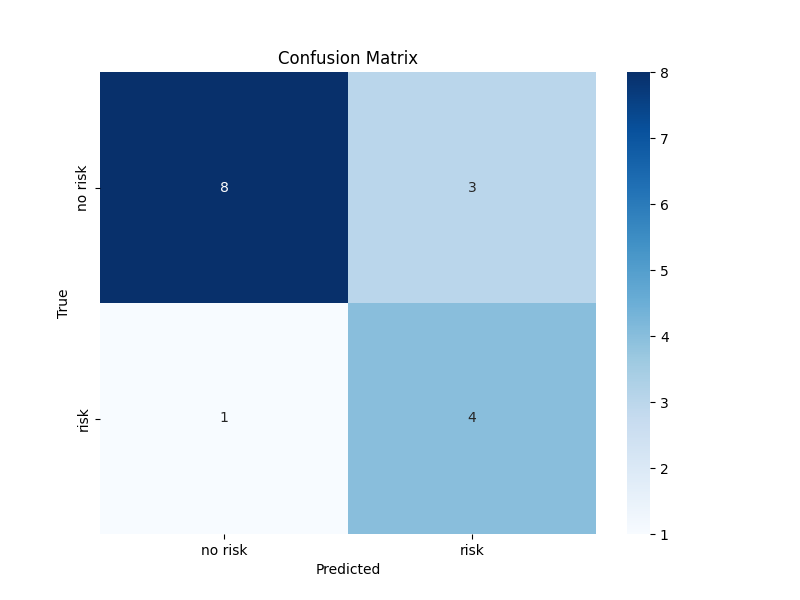
\includegraphics[width=1.0\linewidth]{Master Thesis/Plots/Confusion Matrix risk 1.png}
\caption{Confusion matrix of health risk classification with RF and features maximum heart rate, minimum heart rate and average heart rate, and step count}
\label{fig:ConfusionMatrixrisk1}
\end{figure}
\FloatBarrier

This confusion matrix indicates that the model correctly predicted the 'no risk' class in most cases, but made some errors in predicting the 'risk' class. The precision and recall for both classes reflect this distribution, with higher precision for 'no risk' compared to 'risk'.

The results in general indicate that the model's performance declined compared to the previous version, suggesting that the model places greater importance on non-Apple Watch Ultra data. This was evident when the feature 'age' was removed from the training set, yet the results remained unchanged, indicating that age does not significantly impact this prediction. The decline in performance when incorporating features measured explicitly by the Apple Watch Ultra implies that modifications are necessary to improve the model's effectiveness in utilizing Apple Watch Ultra data for making accurate predictions. This is crucial as our goal is to evaluate how well the data from the Apple Watch Ultra can be used for such predictions.

\subsubsection*{Optimizing the Results of the Random Forest}

To further enhance the results, we utilized the Gradient Boosting Classifier. For this model, we incorporated three heart rate measures (minimum, maximum, and average heart rate over each 6-minute interval of a subject) along with the subject's age, which is not measured by the Apple Watch Ultra. Our aim was to predict the risk by classifying individuals with a BMI over 25 as at-risk. The results using the RF classifier were as following with an accuracy of 0.50:

\begin{table}[H]
\centering
\begin{tabular}{lrrrr}
\toprule
{} & precision & recall & f1-score & support \\
\midrule
no risk & 0.50 & 0.75 & 0.60 & 8.0 \\
risk & 0.50 & 0.25 & 0.33 & 8.0 \\
macro avg & 0.50 & 0.50 & 0.47 & 16.0 \\
weighted avg & 0.50 & 0.50 & 0.47 & 16.0 \\
\bottomrule
\end{tabular}
\caption{RF classification for health risk with features heart rates (minimum, maximum, and average heart rate over each 6-minute interval of a subject) along with the age}
\label{table:thirdtryclass}
\end{table}
The table above ~\ref{table:thirdtryclass} shows the performance metrics for the RF classifier with a lower accuracy. The following confusion matrix visualizes these results:
\FloatBarrier
\begin{figure}[h!]
\centering
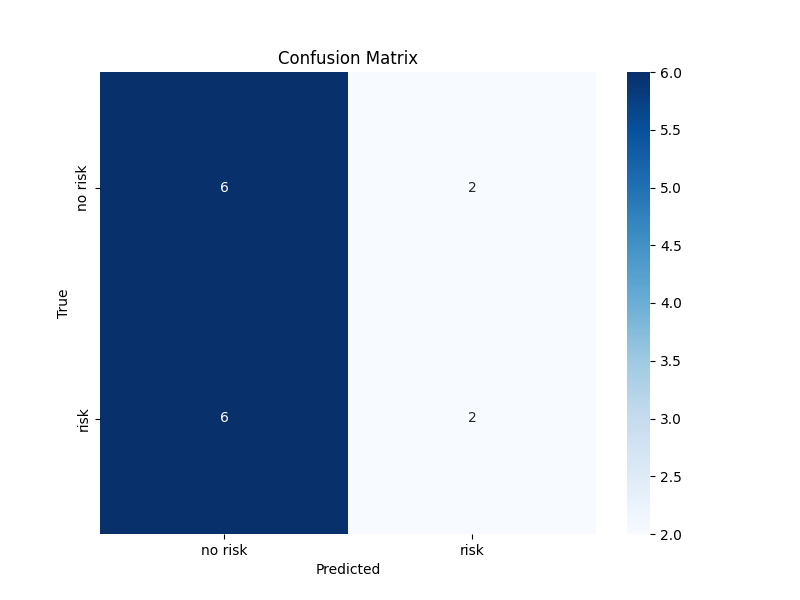
\includegraphics[width=1.0\linewidth]{Master Thesis/Plots/Confusion Matrix risk 2.png}
\caption{Confusion matrix of health risk classification with RF and features heart rates (minimum, maximum, and average heart rate over each 6-minute interval of a subject) along with the age}
\label{fig:ConfusionMatrixrisk2}
\end{figure}
\FloatBarrier

This confusion matrix figure ~\ref{fig:ConfusionMatrixrisk2} demonstrates that the model performs worse in predicting the 'risk' class, as it misclassifies the same number of 'risk' instances as 'no risk' as it correctly classifies. This is confirmed by the lower precision and recall values for the 'risk' class.

The table ~\ref{table:thirdtryclass} shows the performance metrics for the RF Classifier. The precision for both classes is 0.50, indicating that half of the predictions for each class were correct. The recall for class 'no risk' is higher at 0.75, meaning 75\% of the actual class 'no risk' instances were correctly identified, while only 25\% of class 'risk' instances were correctly identified. This imbalance suggests the model is better at identifying non-risk subjects than at identifying at-risk subjects. The f1-scores are 0.60 for class 'no risk' and 0.33 for class 'risk', showing a substantial drop in performance for class 'risk'. The overall accuracy is 50\%, which means the model's predictions are essentially no better than random guessing. The macro average and weighted average f1-scores reflect this poor performance, both at approximately 0.47. These results suggest that the model, in its current form, is not suitable for predicting risk based on the given features.

In contrast, using the gradient boosting classifier, we where able to achieve an accuracy of 0.81 and the following results:

\begin{table}[H]
\centering
\begin{tabular}{lrrrr}
\toprule
{} & precision & recall & f1-score & support \\
\midrule
no risk & 0.78 & 0.88 & 0.82 & 8.0 \\
risk & 0.86 & 0.75 & 0.80 & 8.0 \\
macro avg & 0.82 & 0.81 & 0.82 & 16.0 \\
weighted avg & 0.82 & 0.81 & 0.82 & 16.0 \\
\bottomrule
\end{tabular}
\caption{Gradient boosting classification with features heart rates (minimum, maximum, and average heart rate over each 6-minute interval of a subject) along with the age}
\label{table:boostnr1}
\end{table}

The table ~\ref{table:boostnr1} shows the performance metrics for the gradient boosting classifier. The precision for class 'no risk' is 0.78 and for class 'risk' is 0.86, indicating that the model correctly identifies a high proportion of both non-risk and at-risk subjects. The recall for class 'no risk' is 0.88, meaning 88\% of the actual non-risk instances were correctly identified, while the recall for class 'risk' is 0.75, indicating that 75\% of the actual at-risk instances were correctly identified. The f1-scores are 0.82 for class 'no risk' and 0.80 for class 'risk', reflecting a balanced performance in precision and recall for both classes. The overall accuracy is 81\%, showing a significant improvement compared to the previous model. The macro average and weighted average f1-scores are both at 0.82, demonstrating consistent performance across the dataset. These results suggest that the Gradient Boosting Classifier is more reliable for predicting risk based on the given features.

The RF classifier provided a good initial model for predicting risk among subjects, with promising accuracy and performance metrics. Further optimization using the Gradient Boosting Classifier significantly improved the results, making it a more reliable model for risk prediction in this context.

\subsection{Subject or Patient Classification with Random Forest}

In this subsection, we focus on classifying individuals as either patients (those with health issues) or subjects (healthy individuals). Additionally, we continue to use the previously introduced risk category, for individuals with a BMI over 25, suggesting a higher likelihood of developing health issues. This categorization aims to achieve an even clearer distinction, recognizing that overweight individuals are at increased risk of long-term health problems. The features used in our models include age (not measured by the Apple Watch Ultra) and distance (measured by the Apple Watch Ultra).

Using this set of features (age and distance), the RF model achieved an accuracy of 0.94. Detailed results are shown below:

\FloatBarrier
\begin{table}[H]
\centering
\begin{tabular}{lrrrr}
\toprule
{} & precision & recall & f1-score & support \\
\midrule
patient & 0.91 & 1.00 & 0.95 & 10.00 \\
subject & 1.00 & 0.83 & 0.91 & 6.00 \\
macro avg & 0.95 & 0.92 & 0.93 & 16.00 \\
weighted avg & 0.94 & 0.94 & 0.94 & 16.00 \\
\bottomrule
\end{tabular}
\caption{RF classification with features age and distance}
\label{table:RFageDistance}
\end{table}
\FloatBarrier

The RF model using age and distance features shows excellent performance with an overall accuracy of 0.94. For the 'patient' category, the precision is 0.91, indicating that 91\% of those classified as patients were indeed patients. The recall for this category is 1.00, meaning all actual patients were correctly identified by the model. The f1-score for patients is 0.95, reflecting a balance between precision and recall.

For the 'subject' category, the precision is 1.00, indicating perfect identification of all healthy individuals classified as subjects. The recall for subjects is 0.83, meaning 83\% of actual subjects were correctly identified, with some misclassified as patients. The f1-score for subjects is 0.91.

The macro average f1-score, which is the unweighted mean of the f1-scores for all classes, is 0.93. This suggests that the model performs well across both categories. The weighted average f1-score, which accounts for the number of instances in each class, is 0.94, indicating strong overall model performance.

Using the second set of features (age and heart rate), which includes age (not measured by the Apple Watch Ultra) and heart rate (measured by the Apple Watch Ultra), the model also achieved an accuracy of 0.94:

\FloatBarrier
\begin{table}[H]
\centering
\begin{tabular}{lrrrr}
\toprule
{} & precision & recall & f1-score & support \\
\midrule
patient & 0.91 & 1.00 & 0.95 & 10.00 \\
subject & 1.00 & 0.83 & 0.91 & 6.00 \\
macro avg & 0.95 & 0.92 & 0.93 & 16.00 \\
weighted avg & 0.94 & 0.94 & 0.94 & 16.00 \\
\bottomrule
\end{tabular}
\caption{RF classification with features age and heart rate}
\label{table:RFageHeartrate}
\end{table}
\FloatBarrier

The RF model using age and heart rate features demonstrated high accuracy and effective classification. Precision and recall values were strong for both patient and subject categories, indicating the model's reliability with these features. Specifically, the recall for patients is 1.00, meaning all patient instances were correctly identified. The precision for subjects is 1.00, showing no false positives in identifying subjects.

Using the third set of features (distance and heart rate), both measured by the Apple Watch Ultra, the accuracy dropped to 0.63:

\FloatBarrier
\begin{table}[H]
\centering
\begin{tabular}{lrrrr}
\toprule
{} & precision & recall & f1-score & support \\
\midrule
patient & 0.62 & 1.00 & 0.77 & 10.00 \\
subject & 0.00 & 0.00 & 0.00 & 6.00 \\
macro avg & 0.31 & 0.50 & 0.38 & 16.00 \\
weighted avg & 0.39 & 0.62 & 0.48 & 16.00 \\
\bottomrule
\end{tabular}
\caption{RF classification with features distance and heart rate}
\label{table:RFdistHeartrate}
\end{table}
\FloatBarrier

The model's performance significantly decreased with an accuracy of 0.62 when using only distance and heart rate features. This suggests that these features alone are insufficient for accurate classification. The recall for patients is still high at 1.00, but the precision for subjects is 0.00, indicating the model struggled to correctly classify subjects based on these features alone. This suggests that the model is very dependent on information that the Apple Watch Ultra does not measure and that the results with only Apple Watch Ultra data are simply not meaningful enough.

Incorporating all three features (distance, heart rate, and age), where age is not measured by the Apple Watch Ultra, the model achieved an accuracy of 0.94:

\FloatBarrier
\begin{table}[H]
\centering
\begin{tabular}{lrrrr}
\toprule
{} & precision & recall & f1-score & support \\
\midrule
patient & 0.91 & 1.00 & 0.95 & 10.00 \\
subject & 1.00 & 0.83 & 0.91 & 6.00 \\
macro avg & 0.95 & 0.92 & 0.93 & 16.00 \\
weighted avg & 0.94 & 0.94 & 0.94 & 16.00 \\
\bottomrule
\end{tabular}
\caption{RF classification with features age, heart rate and distance}
\label{table:RFageHeartrateDist}
\end{table}
\FloatBarrier

Including all three features restored the accuracy to 0.94, demonstrating the significance of a comprehensive feature set. The high precision and recall values across both patient and subject categories reinforce the model's reliability and effectiveness. This shows the importance of including multiple relevant features to enhance classification performance, indicating that the model can effectively identify at-risk patients when a broader range of data is used. However, this also leads to the assumption that the model primarily takes into account the age of the test subjects in order to categorize them as sick or healthy.

In summary, the RF model showed consistent high accuracy when age was included as a feature, indicating its crucial role in risk prediction. Conversely, using only the features directly measured by the Apple Watch Ultra (distance and heart rate) resulted in poorer performance. This suggests that while the Apple Watch Ultra provides valuable data, incorporating additional features such as age is essential for improving model accuracy and reliability in predicting health risks.

\subsection{Regression Models}

After using RF, we turned to regression analysis, believing it could help us not only classify data but also predict continuous values accurately. In this section, we explore how close our predictions are to actual values using the RMSE.

We started with linear regression to predict the age of subjects— a feature not measured by the Apple Watch Ultra—using data collected by the watch. Initially, we used height and weight, both not measured by the watch, to establish a baseline model.

Our first linear regression model predicted age with an RMSE of 21.92, showing the average deviation of predicted ages from actual ages. By starting with these features, we set a baseline to evaluate the impact of incorporating Apple Watch Ultra data in improving our predictions. This approach helped us understand which features best predict various health metrics, enhancing our knowledge of the watch's capabilities in health monitoring.

\FloatBarrier
\begin{figure}[h!]
\centering
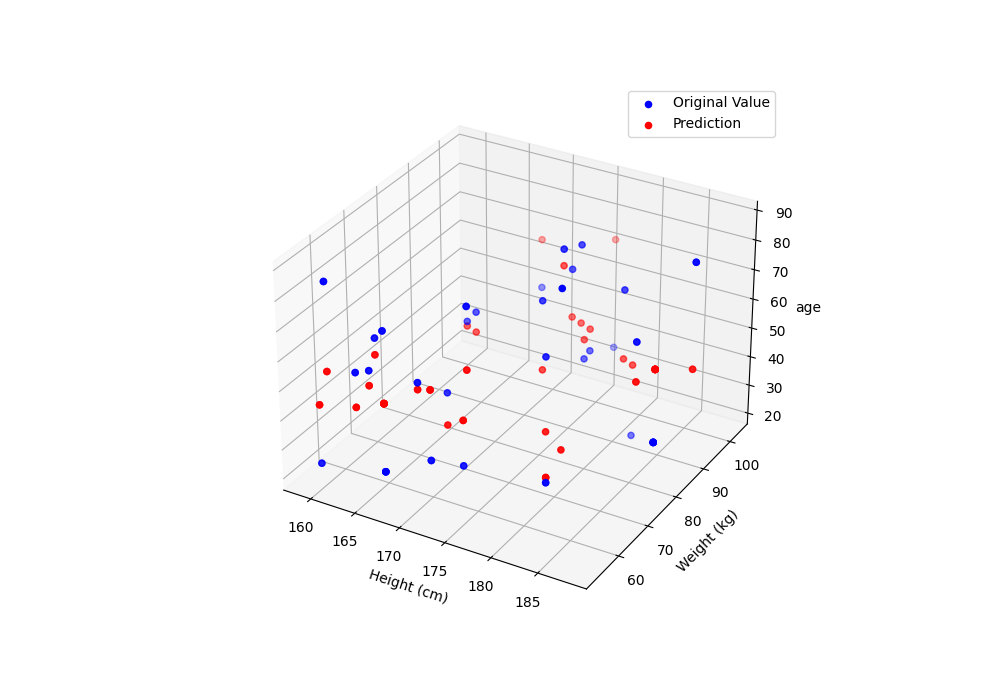
\includegraphics[width=0.9\textwidth]{Master Thesis/Plots/prediction3.png}
\caption{Age prediction with regression based on the features height and weight}
\label{figure:regwithheightweight}
\end{figure}
\FloatBarrier

Figure ~\ref{figure:regwithheightweight} shows a 3D scatter plot comparing actual ages (blue dots) to predicted ages (red dots) based on height and weight. The X-axis represents height in centimeters, the Y-axis shows weight in kilograms, and the Z-axis displays age in years. The closer the red dots are to the blue dots, the more accurate the age predictions by the linear regression model. This plot shows, that the predicted age and original age are quite far apart.

To improve prediction accuracy, we made another attempt with the same linear regression model but with different features. This time, we used leg length, a manually measured feature, and the walked distance, which was measured by the Apple Watch Ultra. Again, we aimed to predict age. This model achieved an RMSE value of 20.76, showing a slight improvement, but the result was still not very accurate.

\FloatBarrier
\begin{figure}[h!]
\centering
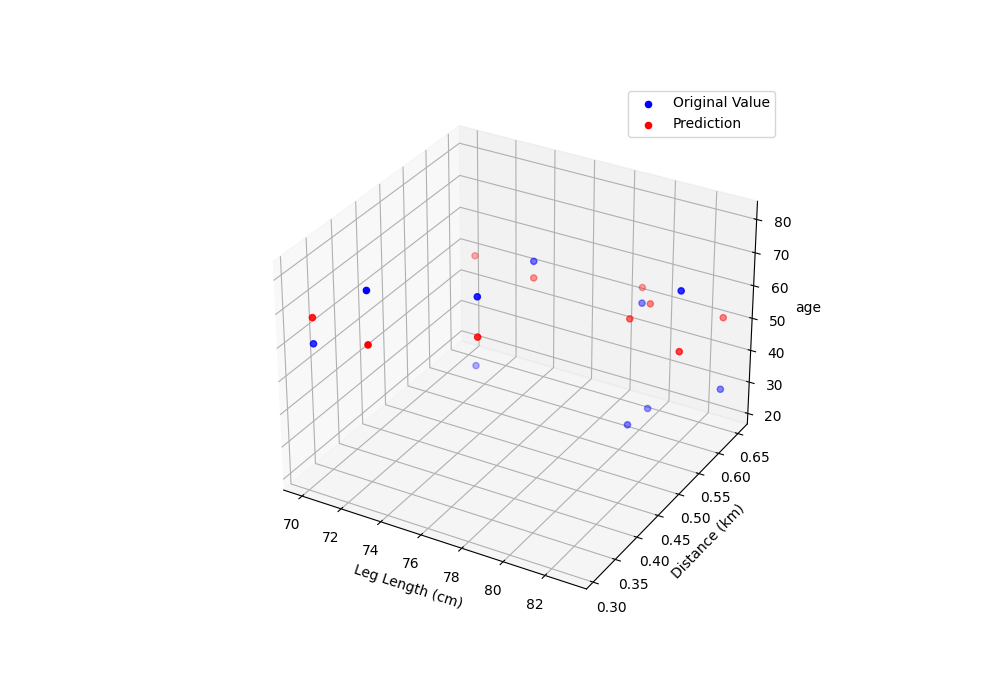
\includegraphics[width=0.9\textwidth]{Master Thesis/Plots/prediction2.png}
\caption{Age prediction with regression based on the leg length and distance}
\label{figure:regwithleglengthdistance}
\end{figure}
\FloatBarrier

Figure ~\ref{figure:regwithleglengthdistance} shows again, that the points are quite far apart from each other, what shows us some potential for optimizing the model or change the features to achieve better results.

While the second model performed better, the high RMSE values indicate that predicting age based solely on these features is challenging, with the predictions being off by over 20 years on average.

\subsubsection*{Expanding the Dataset for Better Predictions}
Recognizing the limitations of predicting age from height and weight alone, we expanded the dataset by including additional features such as heart rates and BMI. This approach aimed to develop more sophisticated models to predict health metrics.

We first attempted to enhance the age prediction model by adding maximum and minimum heart rates, as well as leg length. However, the results were still not very accurate. Believing that regression was still the right tool for such predictions, we next focused on predicting BMI instead of age. By using the feature heart rate (just the minimum value during one interval), we achieved an RMSE of 2.64, which was promising given the typical BMI range of 15 to 40. Further refinements, including using weighted regression with more heart rate data, will be explored later in this study.

\FloatBarrier
\begin{figure}[h!]
\centering
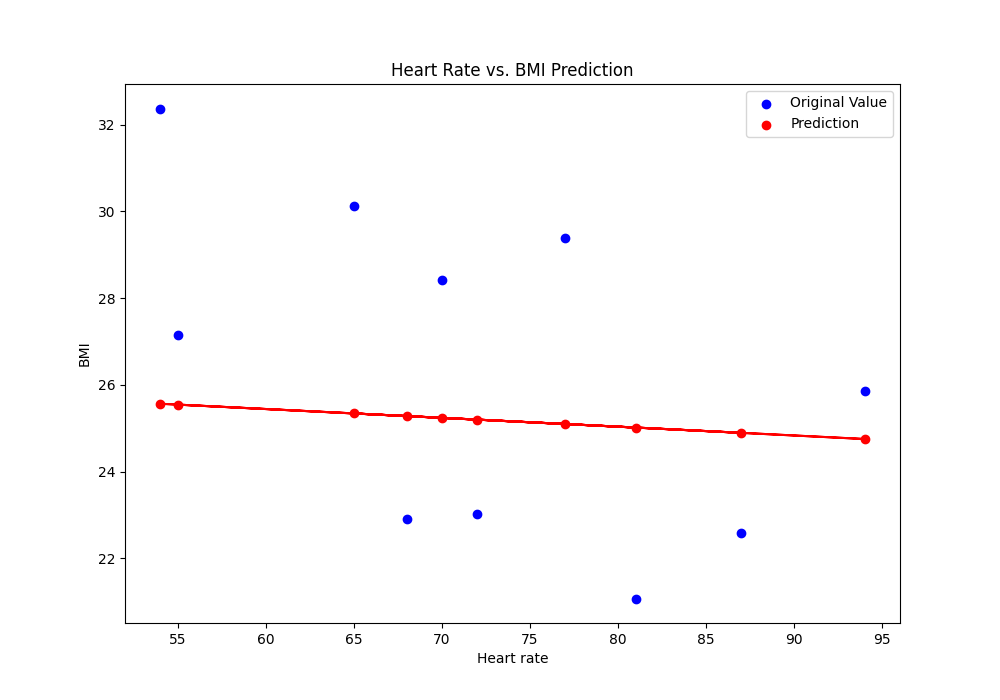
\includegraphics[width=0.6\textwidth]{Master Thesis/Plots/prediction_BMI.png}
\caption{BMI prediction with regression based on heart rate feature}
\label{figure:regwithheartrate}
\end{figure}
\FloatBarrier

The image, labeled as figure ~\ref{figure:regwithheartrate}, is a 2D scatter plot showing the original and predicted BMI values based solely on heart rates. The X-axis represents heart rate, and the Y-axis represents BMI. Red points indicate the original BMI values, while blue points represent the predictions made by the model. The plot shows that the predicted BMI values are randomly distributed around a narrow range, indicating that the model's predictions are not reliable and do not capture the true variability in BMI. The resulting RMSE value was high, suggesting significant prediction errors and demonstrating that heart rates alone are not sufficient to predict BMI accurately.

After initially using only one feature to predict BMI, we decided to incorporate maximum and minimum heart rates along with weight (not measured by the Apple Watch Ultra) as features to improve the prediction. By adding weight as a feature along with heart rates, we achieved a significantly lower RMSE of 1.57. The plot below demonstrates the improved accuracy:

\FloatBarrier
\begin{figure}[h!]
\centering
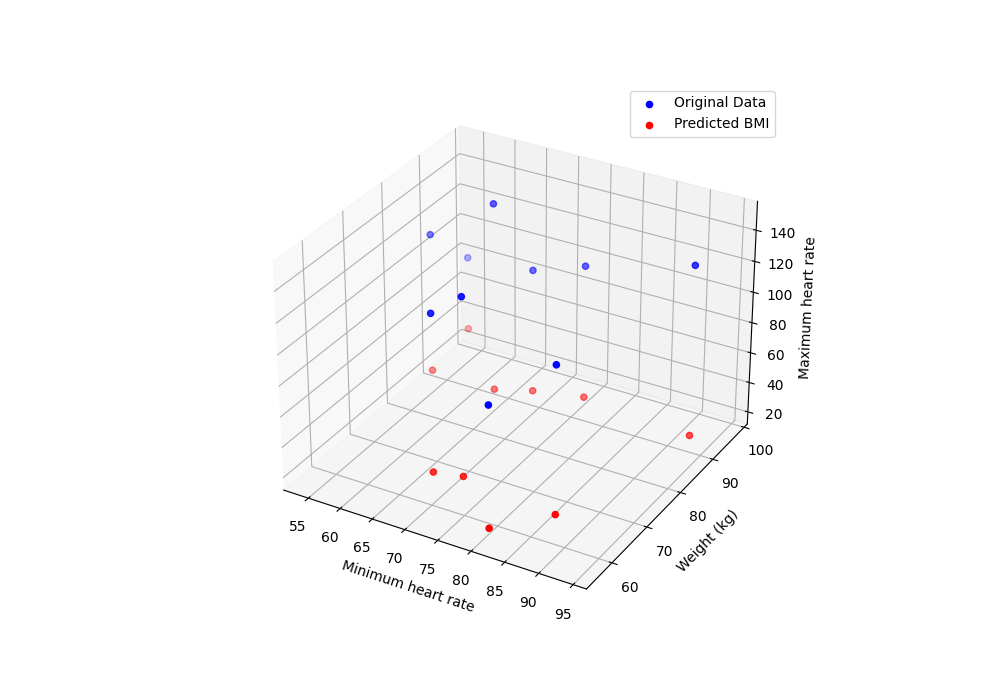
\includegraphics[width=0.9\textwidth]{Master Thesis/Plots/bmi_prediction.png}
\caption{BMI prediction with regression based on features weight and heart rate}
\label{figure:regwithheartrateweight}
\end{figure}
\FloatBarrier

The image, labeled as figure ~\ref{figure:regwithheartrateweight}, is a 3D scatter plot showing the original and predicted BMI values based on both weight and heart rates. The X-axis represents weight (kg), the Y-axis represents heart rate, and the Z-axis represents BMI. Red points indicate the original BMI values, while blue points represent the predictions made by the model. This plot shows a much closer alignment between the original and predicted BMI values, indicating a significant improvement in prediction accuracy. The model achieved a notably lower RMSE value of 1.57, reflecting a substantial reduction in prediction error compared to the previous model.

Although this result is promising, it is important to note that weight is innately included as part of the BMI calculation, making it easier for the model to accurately predict BMI.

With the restructured dataset, included maximum and minimum heart rates, weight, and age as features, we wanted to do another prediction. With these features, we aimed to predict the heart rate using a linear regression model before returning to the subject or patient classification topic using regression.

Using this data, we applied the same linear regression model to predict the actual heart rate based on the weight and age of the subjects. The model achieved an RMSE value of 17.01.

\FloatBarrier
\begin{figure}[h!]
\centering
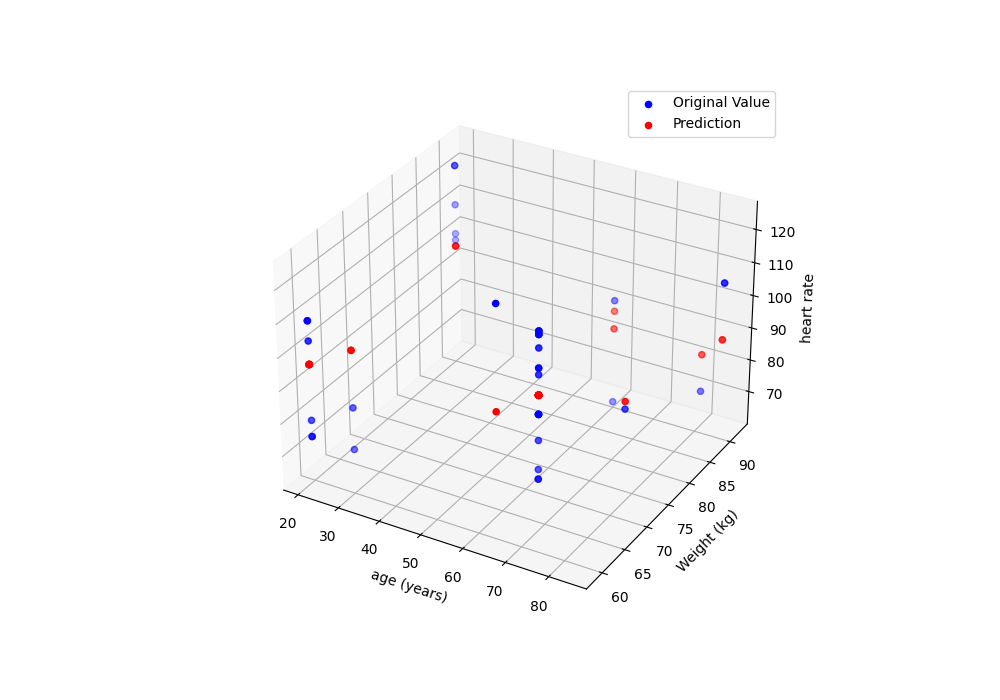
\includegraphics[width=0.9\textwidth]{Master Thesis/Plots/heart-rate_prediction.png}
\caption{Heart rate prediction with regression based on features weight and age}
\label{figure:HRregwithweightage}
\end{figure}
\FloatBarrier

Figure ~\ref{figure:HRregwithweightage} demonstrates a reasonably close alignment between the original and predicted heart rate values, indicating a moderate level of prediction accuracy. The model achieved a RMSE value of 17.01, reflecting the average deviation of the predicted values from the actual values. This RMSE value suggests that while the model's predictions are not perfect, they are within an acceptable range for many applications.

The scatter plot highlights that the model can capture the general trend of how heart rate varies with weight and age, but there are still some discrepancies. These discrepancies could be due to various factors, including the limited number of features used in the model and the inherent variability in heart rate that may be influenced by factors not included in the dataset.

\subsection{Subject or Patient Classification with Logistic Regression}

We used the same dataset from above to evaluate the effectiveness of logistic regression in classifying individuals as either 'patient' or 'subject', based on the risk of developing health issues due to being overweight (BMI over 25) or already being diseased.

Using linear regression, the RMSE was 0.26. Logistic regression yielded to the following results:

\FloatBarrier
\begin{table}[H]
\centering
\begin{tabular}{lcccc}
\toprule
& precision & recall & f1-Score & support \\
\midrule
patient & 0.91 & 1.00 & 0.95 & 10.0 \\
subject & 1.00 & 0.83 & 0.91 & 6.0 \\
macro avg & 0.95 & 0.92 & 0.93 & 16.0 \\
weighted avg & 0.94 & 0.94 & 0.94 & 16.0 \\
\bottomrule
\end{tabular}
\caption{Subject or patient classification with logistic regression based on BMI, heart rate and age}
\label{table:logregpatsubj}
\end{table}
\FloatBarrier

The results from the logistic regression model in table ~\ref{table:logregpatsubj} show a high overall accuracy of 0.94. For the 'patient' category, precision is 0.91, recall is 1.00, and the f1-score is 0.95, indicating that the model correctly identifies all patients but slightly overestimates their count. For the 'subject' category, precision is perfect at 1.00, recall is 0.83, and the f1-score is 0.91, showing that while all identified subjects are correct, some subjects are missed by the model.

The macro average scores, which are the unweighted mean of precision, recall, and f1-score, are also high (0.95, 0.92, and 0.93 respectively), indicating balanced performance across both categories. The weighted average, which accounts for the number of instances in each class, confirms the model's reliability with all metrics at 0.94.

Additionally, the following plots illustrate the predictions made by the logistic regression model and provide an overview of the results:

\FloatBarrier
\begin{figure}[h!]
\centering
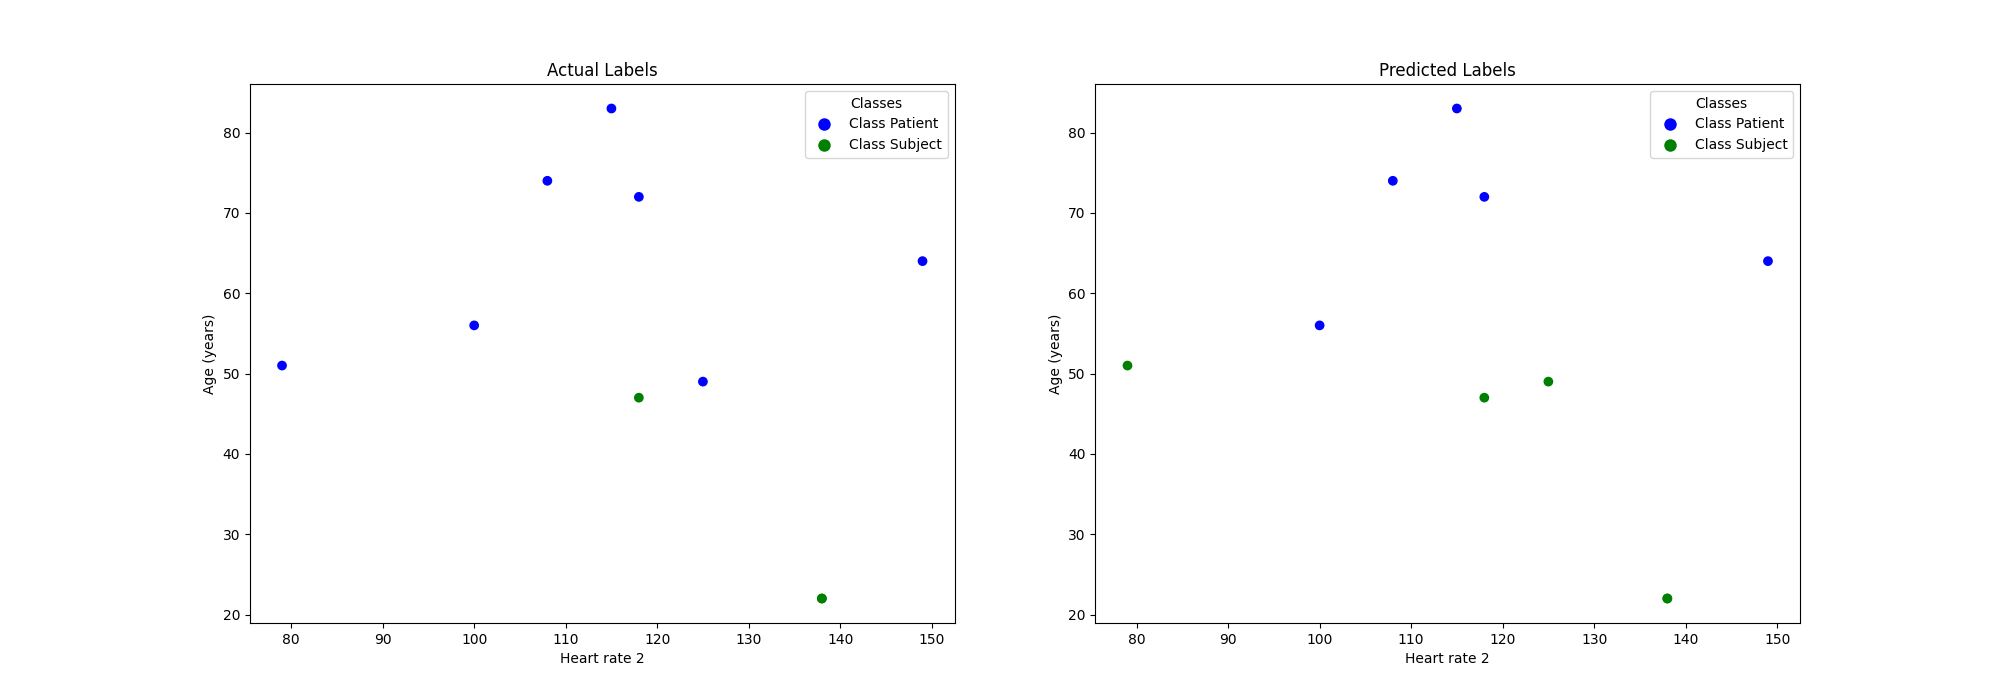
\includegraphics[width=1.1\textwidth]{Master Thesis/Plots/prediction_subjectpatient.png}
\caption{Subject or patient classification with logistic regression based on maximal heart rate and age}
\label{figure:logregwithheartrateage}
\end{figure}
\FloatBarrier

\FloatBarrier
\begin{figure}[h!]
\centering
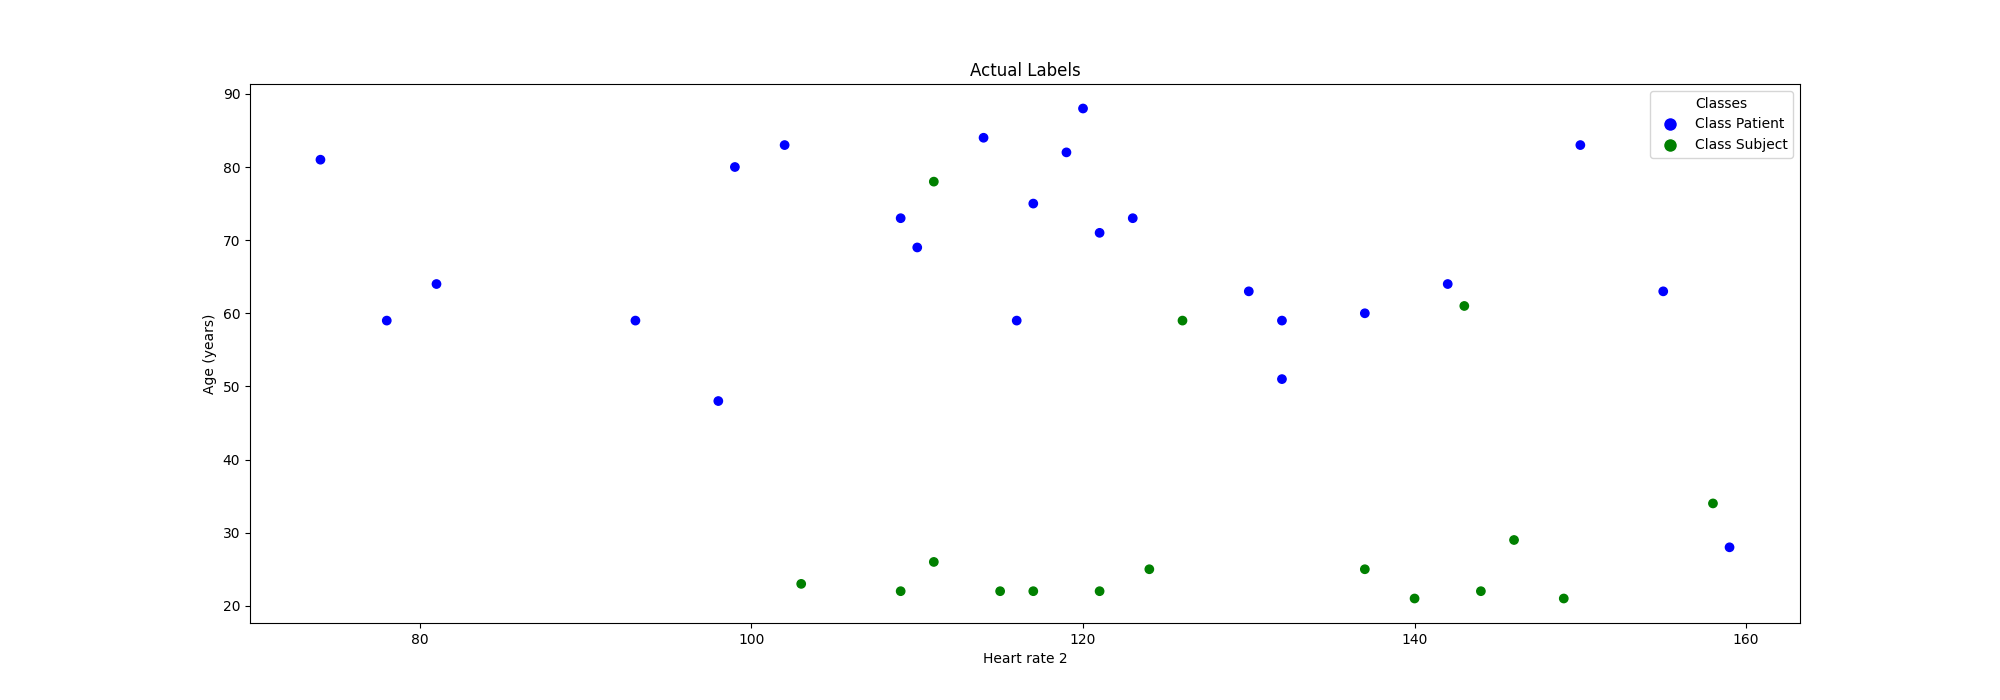
\includegraphics[width=0.9\textwidth]{Master Thesis/Plots/dataset_overview.png}
\caption{Subject or patient classification with logistic regression based on maximal heart rate and age all data}
\label{figure:logregwithheartrateageall}
\end{figure}
\FloatBarrier

The first two plots in figure ~\ref{figure:logregwithheartrateage} display the actual and predicted labels of 'subject/patient' status based on age and heart rate. The plot on the left shows the actual labels, where blue dots represent subjects and green dots represent patients. The plot on the right shows the predicted labels by the logistic regression model, similarly colored. The alignment of blue and green dots between the two plots indicates the model's accuracy in predicting the correct category.

Figure ~\ref{figure:logregwithheartrateageall} provides a comprehensive overview of the dataset, showing the distribution of subjects and patients based on age and heart rate. Each dot represents an individual, with blue dots indicating subjects and green dots indicating patients. This visualization helps in understanding the spread and clustering of the data points, as well as the relationship between age, heart rate and health status.

\subsection{Neural Networks}

In the methodology chapter ~\ref{cha:methods}, we introduced neural networks and aimed to test their suitability for this dataset. We considered various combinations of features to evaluate the deep learning models, which aimed to predict physiological measurements based on age and exercise behavior. Specifically, the models focused on predicting heart rate from age and walked distance. Additionally predicting walked distance from age and heart rate. And finally predicting age from heart rate and walked distance:

\FloatBarrier
\begin{table}[htbp]
\centering
\begin{tabular}{@{}lcc@{}}
\toprule
\textbf{model description} & \textbf{MSE} & \textbf{interpretation} \\ \midrule
heart rate prediction (age, distance) & 1.10 & moderate error \\
distance prediction (age, heart rate) & \textbf{0.59} & low error \\
age prediction (heart rate, distance) & 0.60 & low error \\ 
\bottomrule
\end{tabular}
\caption{Performance of deep learning models measured in MSE for different features}
\end{table}
\FloatBarrier

The model predicting heart rate based on age and distance achieved a MSE of 1.10, indicating a moderate level of error. This suggests that while age and distance have some predictive power, additional factors likely influence heart rate that are not captured by these two variables alone.

Predicting distance walked based on age and heart rate resulted in a low MSE of 0.59. This low error indicates a strong relationship between these variables, implying that the model can accurately predict distance traveled with the given inputs. This suggests good predictive accuracy and a strong link between physical activity, age, and heart rate.

The model predicting age based on heart rate and distance traveled achieved an MSE of 0.60. The low error suggests that these two features provide valuable information about the biological age of an individual, which could highlight discrepancies between biological and chronological age based on fitness data.

We then applied a slightly modified version of the same deep learning model, focusing on visualizing the results and calculating accuracy instead of the MSE. 

\FloatBarrier
\begin{figure}[h!]
\centering
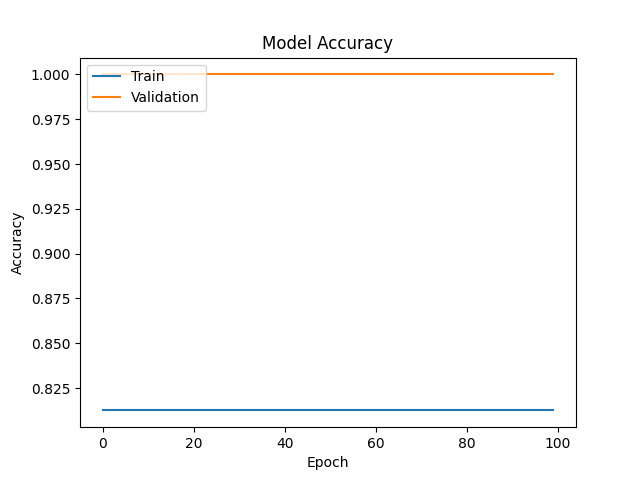
\includegraphics[width=0.8\textwidth]{Master Thesis/Plots/deepLearningModel_age+heartRate1.png}
\caption{Accuracy of deep learning model}
\label{figure:modelaccNN}
\end{figure}
\FloatBarrier

\FloatBarrier
\begin{figure}[h!]
\centering
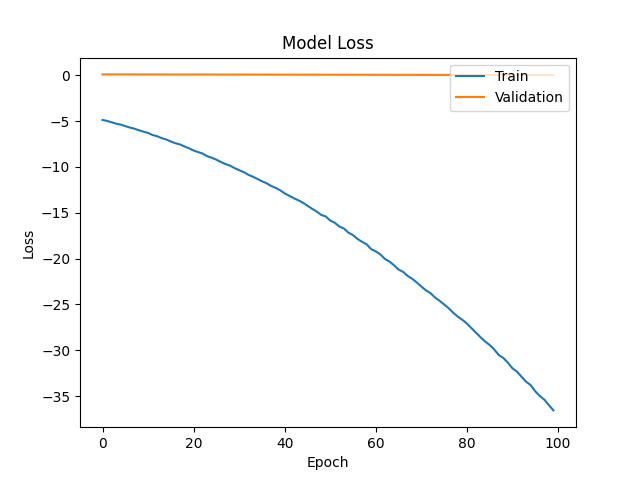
\includegraphics[width=0.8\textwidth]{Master Thesis/Plots/deepLearningModel_age+heartRate2.png}
\caption{Loss of deep learning model}
\label{figure:modellossNN}
\end{figure}
\FloatBarrier

Using the features of age and heart rate, the model achieved an accuracy of 81.25\%. This means that the model correctly predicted or classified 81.25$\%$ of the test dataset, indicating a strong performance. 

Figure ~\ref{figure:modelaccNN} shows the model accuracy, with the X-axis representing the number of epochs and the Y-axis representing the accuracy. The blue line indicates the training accuracy, and the orange line indicates the validation accuracy. The plot reveals that the training accuracy remains constant and low throughout the epochs, suggesting that the model is not improving its performance on the training data. In contrast, the validation accuracy is constant and perfect (1.0) from the beginning. This unusual behavior may indicate a potential issue in the training process.

Figure ~\ref{figure:modellossNN} displays the model loss, with the X-axis denoting the number of epochs and the Y-axis denoting the loss value. The blue line represents the training loss, and the orange line represents the validation loss. The training loss consistently decreases over the epochs, indicating that the model is learning and fitting the training data progressively better. However, the validation loss remains constant and does not show any improvement, which is unusual given that the validation accuracy was perfect in Figure 7.8. This suggests a discrepancy between the loss and accuracy metrics or a possible issue in the loss calculation or data handling. 

\section{Unsupervised Learning Models}

In this section, we aim to evaluate the performance of unsupervised learning models, specifically focusing on clustering, on our dataset. The goal is to determine how well this method can group similar data points based on the collected health metrics.

\subsection{Clustering Method}

Using the same dataset as in the whole chapter ~\ref{cha:results}, we aimed to evaluate how well the data can be clustered using unsupervised learning techniques. We specifically applied k-means clustering and hierarchical clustering using the features age and heart rate.

The quality of the clusters was assessed using silhouette scores and Davies-Bouldin scores. For k-means clustering, a silhouette score of 0.27 was obtained. This low score indicates that the clusters are not well-formed, with significant overlap or dispersion among data points. Ideally, a silhouette score close to 1 suggests well-defined clusters, while a score around -1 indicates incorrect clustering.

Additionally, the Davies-Bouldin score for k-means clustering was 1.28. Lower Davies-Bouldin scores indicate better cluster separation, with an ideal value being 0. The score of 1.28 suggests that the clusters have poor separation and high variance within them.

These two plots were generated to visualize the clusters:

\FloatBarrier
\begin{figure}[h!]
\centering
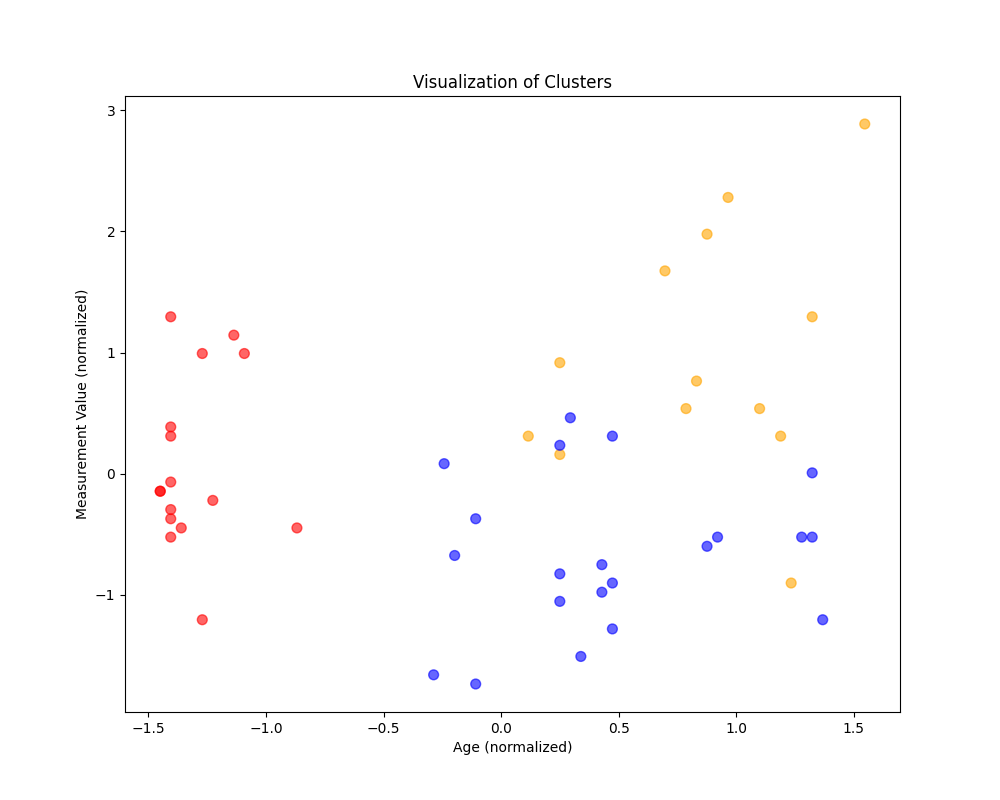
\includegraphics[width=0.9\textwidth]{Master Thesis/Plots/cluster_visualization_no_yellow.png}
\caption{Clustering visualization with features age and heart rate}
\label{figure:clusterageHR}
\end{figure}

\begin{figure}[h!]
\centering
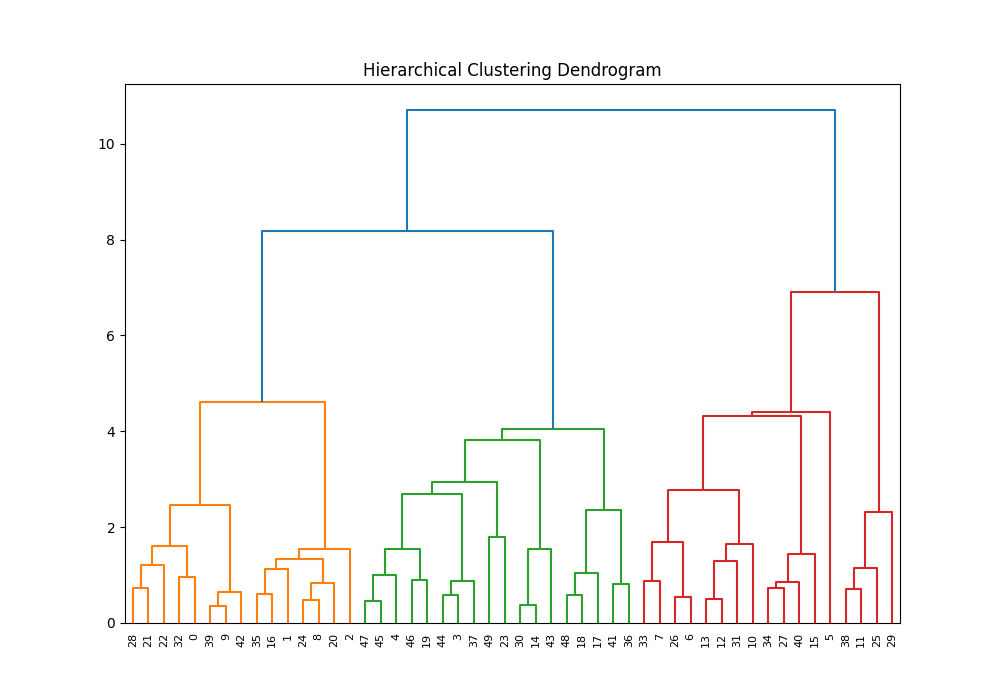
\includegraphics[width=0.9\textwidth]{Master Thesis/Plots/HierarchicalClustering_age+heartRate.png}
\caption{Hierarchical clustering visualization with features age and heart rate}
\label{figure:hirclusterageHR}
\end{figure}
\FloatBarrier

For hierarchical clustering, a silhouette score of 0.27 and a Davies-Bouldin score of 1.42 were obtained. The silhouette score, similar to the k-means result, indicates moderate clustering quality, with clusters that are not very compact or well-separated. The Davies-Bouldin score of 1.42 further indicates that the clusters are not optimally separated, suggesting average cluster separation and compactness.

The first figure ~\ref{figure:clusterageHR} shows the k-means clustering results, where the clusters are represented with different colors. The dispersion and overlap of points suggest that the clusters are not well-defined. The second figure ~\ref{figure:hirclusterageHR} illustrates the hierarchical clustering dendrogram, highlighting the relationships and distances between data points. The dendrogram shows that the clusters are not clearly separated, which is consistent with the silhouette and Davies-Bouldin scores.

Overall, the clustering results for both methods reveal that the features age and heart rate do not form well-defined clusters within the dataset. This could be attributed to the nature of the data, the choice of features, or the clustering method used. Further refinement in feature selection or alternative clustering approaches may be needed to achieve better-defined clusters but at this point we wanted to try other models as well.

\section{Analyzing the 6MWT Theory}

The aim of this section is to explore the correlation between age, distance, and heart rate using various classification and regression models. This analysis proofs or disproofs the hypothesis that age and heart rate can predict the distance traveled by subjects, which is central to the 6MWT theory.

\subsection{SVM Learning Model for 6MWT Features}

In this subsection, we investigate the potential of SVM learning to classify features associated with the 6MWT. The 6MWT is a widely used test to assess functional performance and predict cardiovascular and respiratory diseases by measuring the distance an individual can quickly walk on a flat, hard surface in six minutes. This test can also be used to determine the age of the subject based on the distance walked and the heart rate, and to intervene if the determined age differs too much from the calculated age. By analyzing our dataset, we aim to evaluate how well SVM models can predict health features based on the data collected during the 6MWT.

To explore the effectiveness of SVM learning for this purpose, various feature sets were tested. Using the first set of features, age and walked distance, the SVM model achieved an accuracy of 0.63. The detailed results are shown in the table below:

\FloatBarrier
\begin{table}[H]
\centering
\begin{tabular}{lrrrr}
\toprule
{} & precision & recall & f1-score & support \\
\midrule
no risk & 1.00 & 0.45 & 0.62 & 11.00 \\
risk & 0.45 & 1.00 & 0.62 & 5.00 \\
macro avg & 0.73 & 0.73 & 0.62 & 16.00 \\
weighted avg & 0.83 & 0.62 & 0.62 & 16.00 \\
\bottomrule
\end{tabular}
\caption{SVM model results with features age and distance}
\label{table:svmagedist}
\end{table}
\FloatBarrier

The SVM model's performance using age and distance as features yielded an overall accuracy of 0.62. For class 'no risk', the model achieved a perfect precision of 1.00, indicating it correctly identified all instances it classified as no risk. However, the recall for class 'no risk' was only 0.45, meaning the model missed more than half of the actual no-risk instances. Conversely, for class 'risk', the precision was 0.45, indicating a substantial number of false positives. The recall for class 'risk' was 1.00, showing that the model correctly identified all risk instances but at the cost of many false alarms. The macro average precision and recall were both 0.73, reflecting the model's mixed performance across the two classes, while the weighted averages highlight the same trend, emphasizing the imbalance in classification accuracy.

For the second set of features we used the age and the heart rate of the subjects. The SVM model also resulted in an accuracy of 0.63. The results are summarized in the following table:

\FloatBarrier
\begin{table}[H]
\centering
\begin{tabular}{lrrrr}
\toprule
{} & precision & recall & f1-score & support \\
\midrule
no risk & 1.00 & 0.45 & 0.62 & 11.00 \\
risk & 0.45 & 1.00 & 0.62 & 5.00 \\
macro avg & 0.73 & 0.73 & 0.62 & 16.00 \\
weighted avg & 0.83 & 0.62 & 0.62 & 16.00 \\
\bottomrule
\end{tabular}
\caption{SVM model results with features age and heart rate}
\label{table:svmageHR}
\end{table}
\FloatBarrier

Using age and heart rate as features, the SVM model achieved an accuracy of 0.62, mirroring the results obtained with age and distance. The precision for class 'no risk' remained perfect at 1.00, but the recall was low at 0.45, indicating the model effectively identified true negatives but missed many true positives. For class 'risk', the precision was 0.45, reflecting a significant number of false positives, while the recall was 1.00, indicating the model correctly identified all risk instances. The macro average precision and recall scores were both 0.73, similar to the previous feature set, highlighting the consistent but limited predictive power of the model. The weighted averages further illustrate the model's imbalance in performance across the two classes.

When we changed the features to distance and heart rate, the accuracy improved to 0.69, as shown in the following table:

\FloatBarrier
\begin{table}[H]
\centering
\begin{tabular}{lrrrr}
\toprule
{} & precision & recall & f1-score & support \\
\midrule
no risk & 0.69 & 1.00 & 0.81 & 11.00 \\
risk & 0.00 & 0.00 & 0.00 & 5.00 \\
macro avg & 0.34 & 0.50 & 0.41 & 16.00 \\
weighted avg & 0.47 & 0.69 & 0.56 & 16.00 \\
\bottomrule
\end{tabular}
\caption{SVM Results with Distance and Heart Rate}
\end{table}
\FloatBarrier

The combination of distance and heart rate improved the accuracy to 0.69. However, the recall for class 'risk' was zero, indicating that it failed to correctly identify any of the positive cases. This suggests that while the model can identify non-risk cases effectively, it struggles to detect risk cases using these features. The precision for class 'no risk' was 0.69 with a recall of 1.00, meaning the model identified all true negatives but failed to identify true positives for class 'risk'. The macro average indicates that the overall model performance is poor in detecting risk cases, emphasizing the need for better feature selection or model adjustment.

Finally, by incorporating all three features (distance, heart rate and age), the SVM model maintained an accuracy of 0.63, as shown in the table below:

\FloatBarrier
\begin{table}[H]
\centering
\begin{tabular}{lrrrr}
\toprule
{} & precision & recall & f1-score & support \\
\midrule
no risk & 1.00 & 0.45 & 0.62 & 11.00 \\
risk & 0.45 & 1.00 & 0.62 & 5.00 \\
macro avg & 0.73 & 0.73 & 0.62 & 16.00 \\
weighted avg & 0.83 & 0.62 & 0.62 & 16.00 \\
\bottomrule
\end{tabular}
\caption{SVM model results with features age, heart rate and distance}
\label{table:svmageHRdist}
\end{table}
\FloatBarrier

Including all three features (distance, heart rate and age) did not improve the accuracy, maintaining it at 0.62. The precision and recall values remained consistent with previous tests, indicating that the additional feature did not contribute significantly to the model's predictive capability. This suggests that while the model is effective in identifying non-risk cases, it struggles with detecting risk cases even with the inclusion of an additional feature.

When the feature 'leg length (cm)' was added, the performance worsened, with accuracy dropping to 0.50 across all sets. This indicates that including irrelevant or weakly correlated features can degrade the model's performance, highlighting the importance of feature selection in predictive modeling.

\subsection{Random Forest Model for 6MWT Features}

To classify the risk of subjects based on measured heart rate, distance, and age, the same model was used as in the previous subsection on RF with a few improvements. The features used in the initial model included heart rate and distance (measured by the Apple Watch Ultra), along with age (not measured by the Apple Watch Ultra). The model aimed to predict the risk classification of subjects without considering BMI.

The initial set of features resulted in an accuracy of 63\%. Detailed results are shown in the table below:

\begin{table}[H]
\centering
\begin{tabular}{lrrrr}
\toprule
{} & precision & recall & f1-score & support \\
\midrule
no risk & 0.58 & \textbf{0.88} & 0.70 & 8.00 \\
risk & \textbf{0.75} & 0.38 & 0.50 & 8.00 \\
macro avg & 0.67 & 0.63 & 0.60 & 16.00 \\
weighted avg & 0.67 & 0.63 & 0.60 & 16.00 \\
\bottomrule
\end{tabular}
\caption{RF classification with features distance, heart rate and age}
\label{table:RFdistHeartrateage}
\end{table}

The initial results in table ~\ref{table:RFdistHeartrateage} show moderate performance. The precision for the positive class 'risk' is 0.75, indicating that 75\% of the predicted positives are true positives. For the negative class 'no risk', the precision is 0.58. The recall for the negative class is high at 0.88, meaning the model correctly identifies 88\% of the true negatives. However, the recall for the positive class is low at 0.38, indicating that the model misses many true positives. The overall accuracy is 63\%, showing some predictive capability but room for improvement.

To further explore the impact of different features on model performance, several variations were tested. Initially, only heart rate and age were used, resulting in an accuracy of 50\%, indicating randomness and insufficient predictive power.

After that, we wanted to see if reducing the number of features might improve the results, so we used only age and distance. This approach led to an improved accuracy of 81\%, as shown in the table below:

\begin{table}[H]
\centering
\begin{tabular}{lrrrr}
\toprule
{} & precision & recall & f1-score & support \\
\midrule
no risk & 0.73 & \textbf{1.00} & 0.84 & 8.00 \\
risk & \textbf{1.00} & 0.63 & 0.77 & 8.00 \\
Macro Avg & 0.86 & 0.81 & 0.81 & 16.00 \\
Weighted Avg & 0.86 & 0.81 & 0.81 & 16.00 \\
\bottomrule
\end{tabular}
\caption{RF classification with features distance and age}
\label{table:RFdistage}
\end{table}

The results in table ~\ref{table:RFdistage} indicate a significant improvement, with an accuracy of 81\%. The precision for the positive class increased to 1.00, and the recall for the negative class remained perfect at 1.00, suggesting that age and distance are strong predictors for risk classification.

Interestingly, omitting heart rate data and using only age and distance improved the model's performance, suggesting that the heart rate data from the Apple Watch Ultra might not contribute significantly to risk prediction in this context. This implies that the model can achieve better results without relying on Apple Watch Ultra data, emphasizing the robustness of age and distance as key predictive features.

Testing with heart rate and distance again yielded an accuracy of 50\%, confirming the randomness of this feature set. This further highlights the potential inadequacy of heart rate data from the Apple Watch Ultra for effective risk prediction in this specific application.

\subsubsection{Optimizing the Random Forest Model}

To improve the accuracy of the RF model, we used Grid Search Cross-Validation (CV) to find the best hyperparameters. This process involved trying different combinations of features to find the most effective settings. The table below shows the optimization results, where negative scores represent the negative MSE. A lower score means better model performance.

\FloatBarrier
\begin{table}[h!]
\centering
\label{tab:optimization_results}
\begin{tabular}{>{\raggedright\arraybackslash}p{3.5cm} >{\raggedright\arraybackslash}p{6cm} r}
\toprule
\textbf{feature set} & \textbf{best parameters} & \textbf{best score} \\
\midrule
heart rate and distance & \texttt{max\_depth: None, max\_features: 'sqrt', min\_samples\_leaf: 1, min\_samples\_split: 10, n\_estimators: 200} & -0.4167 \\
\addlinespace
\textbf{age and distance} & \texttt{max\_depth: None, max\_features: 'sqrt', min\_samples\_leaf: 1, min\_samples\_split: 2, n\_estimators: 100} & \textbf{-0.2667} \\
\addlinespace
heart rate and age & \texttt{max\_depth: None, max\_features: 'sqrt', min\_samples\_leaf: 4, min\_samples\_split: 2, n\_estimators: 200} & -0.2833 \\
\addlinespace
\textbf{heart rate, distance, and age} & \texttt{max\_depth: None, max\_features: 'sqrt', min\_samples\_leaf: 1, min\_samples\_split: 2, n\_estimators: 100} & \textbf{-0.2667} \\
\bottomrule
\end{tabular}
\caption{RF optimization results with CV and different feature sets}
\label{table:RFoptiCV}
\end{table}
\FloatBarrier

The RF model includes several key hyperparameters that control its behavior and performance. The 'max\_depth' parameter limits the maximum depth of the trees, preventing overfitting by restricting the model's complexity. The 'max\_features' parameter dictates the number of features to consider when looking for the best split, which introduces randomness and reduces the risk of overfitting. The 'min\_samples\_leaf' parameter sets the minimum number of samples required to be at a leaf node, ensuring that each leaf has enough data to avoid learning from noise. The 'min\_samples\_split' parameter specifies the minimum number of samples needed to split an internal node, preventing splits that create overly specific branches. Lastly, the 'n\_estimators' parameter determines the number of trees in the forest, balancing model accuracy and computational efficiency by controlling the number of decision trees built in the RF. Properly tuning these hyperparameters is essential for developing a robust and well-generalizing RF model.

The table lists the best parameters and the corresponding scores for various feature combinations, highlighting the performance of each set measured and compared trough their MSE.

The feature set combining age and distance achieved the best performance, with a score of -0.2667. This indicates that these features are highly effective for the model, as reflected in the lowest negative mean squared error. The feature set incorporating heart rate, distance, and age also achieved the same best score of -0.2667, reinforcing the importance of age and distance in the model's predictions.

In contrast, the feature set of heart rate and distance yielded the worst performance with a score of -0.4167, suggesting that these features alone are less effective for accurate classification. The set of heart rate and age performed better than heart rate and distance but was still not as effective as age and distance alone, with a score of -0.2833.

In conclusion, the RF model's optimization results demonstrate that using age and distance as features provides the best classification accuracy. The hyperparameter tuning further enhanced the model's performance, indicating the significance of these features in predicting the risk of subjects. Future analysis will explore the impact of excluding data from certain devices, such as the Apple Watch Ultra, to understand potential limitations and improve the model's predictions.

\subsection{Regression Model for 6MWT Features}

We aimed to see if regression could yield better results than our previous models. Initially, we used age and heart rate as predictors to estimate the distance traveled by subjects. The resulting RMSE was 7.26, indicating that the predictions deviated from the actual values by approximately seven meters, which is relatively accurate.

\FloatBarrier
\begin{figure}[h!]
    \centering
    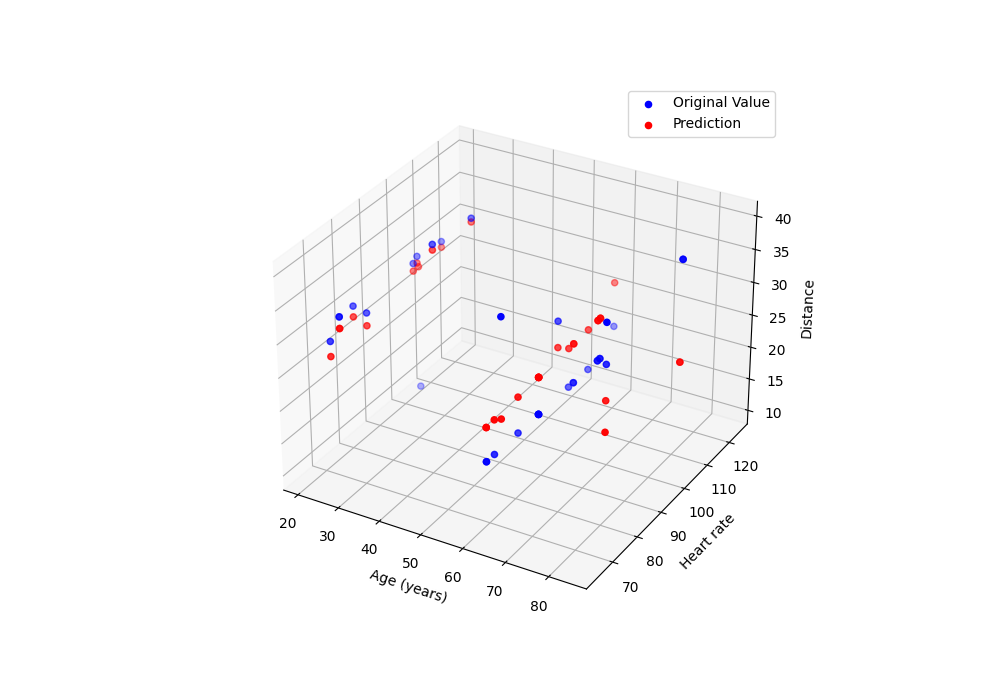
\includegraphics[width=0.9\textwidth]{Master Thesis/Plots/Distance_prediction.png}
    \caption{Distance prediction with regression based on features heart rate and age}
\label{figure:distregwithHRage}
\end{figure}
\FloatBarrier

Figure ~\ref{figure:distregwithHRage} shows a 3D scatter plot with age (years) on the X-axis, heart rate on the Z-axis, and distance on the Y-axis. The scatter plot visually demonstrates the alignment between the original and predicted values, indicating a moderate level of accuracy in the regression model. The dots are close to each other, what corresponds to our lower RMSE value.

To further improve the accuracy of the model, we applied gradient boosting regression. This approach resulted in a lower RMSE value of 4.65. Furthermore, this shows that the accuracy of the model varies by about 1.26 meters in different parts of the dataset. This variation suggests that the model performs more consistently in some scenarios or for certain patient groups.
We obtained this diagram: 

\FloatBarrier
\begin{figure}[h!]
    \centering
    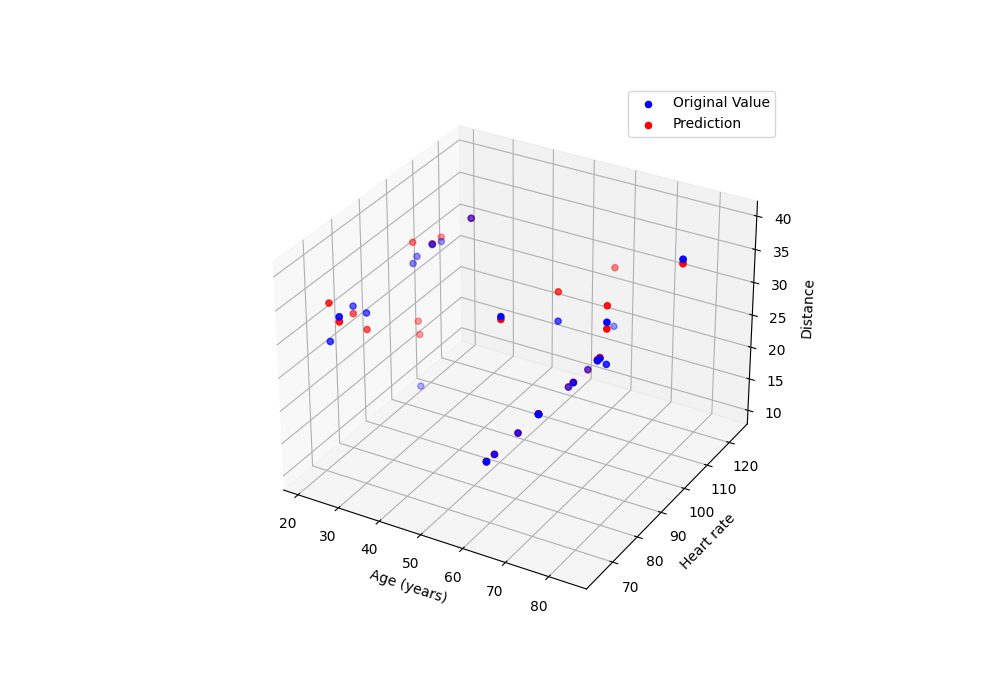
\includegraphics[width=0.9\textwidth]{Master Thesis/Plots/Proof_6MWT_prediction.png}
    \caption{Distance prediction with gradient boosting regression based on features heart rate and age}
    \label{figure:distGBregwithHRage}
\end{figure}
\FloatBarrier

Figure ~\ref{figure:distGBregwithHRage} shows a 3D scatter plot with again age (years) on the X-axis, heart rate on the Z-axis, and distance on the Y-axis. The scatter plot visually demonstrates the alignment between the original and predicted values, indicating a even better level of accuracy in the regression model. The dots are even closer to each other, what corresponds to our smaller RMSE value.

The GBR model outperforms the simple linear regression, as indicated by the tighter clustering of predicted points around the actual values and a lower RMSE value. These results suggest that using more sophisticated regression techniques can lead to more accurate predictions, supporting the correlation between age, heart rate, and distance traveled in the context of the 6MWT theory.

\subsubsection*{Model Performance Evaluation}

In this part of the work, we aim to verify the hypothesis from the previous section that boosting regression model might perform better for our dataset. Therefore, we will evaluate the performance of various regression models (linear regression, gradient boosting, XGBoost, CatBoost, and ensemble models) for each feature: heart rate, age and distance. Our analysis will focus on determining which model yields the best results for each feature by comparing their RMSE values.

The RMSE will be our primary metric for assessing model accuracy. RMSE measures the differences between values predicted by a model and the actual observed values, providing a clear indication of the model's prediction accuracy.

\subsubsection*{Heart Rate Prediction} 

\FloatBarrier
\begin{table}[htbp]
\centering
\begin{tabular}{@{}lc@{}}
\toprule
model & RMSE \\ 
\midrule
linear regression & \textbf{17.30} \\
gradient boosting regression & 19.62 \\
XGBoost regression & 18.77 \\
CatBoost regression & 17.60 \\
ensemble regression & 18.45 \\ 
\bottomrule
\end{tabular}
\caption{RMSE results for predicting heart rate feature with different regression models}
\end{table}
\FloatBarrier

The results indicate that the linear regression model performs the best in predicting heart rate, with an RMSE of 17.30. CatBoost regression follows closely with an RMSE of 17.60. The gradient boosting and XGBoost models shows slightly higher RMSE values of 19.62 and 18.77, respectively, indicating less accuracy compared to linear regression. The ensemble regression model performs moderately with an RMSE of 18.45.

\subsubsection*{Age Prediction} 
\FloatBarrier
\begin{table}[htbp]
\centering
\begin{tabular}{@{}lc@{}}
\toprule
model & RMSE\\ \midrule
linear regression & 21.50 \\
gradient boosting regression & 13.31 \\
XGBoost regression & 12.98 \\
CatBoost regression & \textbf{12.37} \\
ensemble regression & 12.59 \\ \bottomrule
\end{tabular}
\caption{RMSE results for predicting age feature with different regression models}
\end{table}
\FloatBarrier

The CatBoost regression achieves the lowest RMSE of 12.37, making it the most accurate model for predicting age. The XGBoost regression model closely follows with an RMSE of 12.98. Gradient boosting regression also performs well with an RMSE of 13.31. The linear regression model shows a significantly higher RMSE of 21.50, indicating less accuracy. The ensemble regression model has a decent performance with an RMSE of 12.59.

\newpage
\subsubsection*{Distance Prediction}
\FloatBarrier
\begin{table}[htbp]
\centering
\begin{tabular}{@{}lc@{}}
\toprule
model & RMSE \\ \midrule
linear regression & 7.26 \\
gradient boosting regression & 4.65 \\
XGBoost regression & \textbf{3.27} \\
CatBoost regression & 4.24 \\
ensemble regression & 3.62 \\ \bottomrule
\end{tabular}
\caption{RMSE results for predicting distance feature with different regression models}
\end{table}
\FloatBarrier

For distance prediction, the XGBoost regression model outperforms all others with the lowest RMSE of 3.27. The ensemble regression model also demonstrates high accuracy with an RMSE of 3.62. CatBoost regression and gradient boosting regression follow with RMSE values of 4.24 and 4.65, respectively. Linear regression has the highest RMSE of 7.26, indicating it was the least accurate model for this task.

The results of the regression model evaluations highlight that boosting models, particularly XGBoost and CatBoost, often provide superior performance compared to linear regression. For heart rate prediction, linear regression performed the best, whereas for age and distance predictions, boosting models outperformed others. This reinforces the importance of selecting appropriate models for different features to achieve the best predictive accuracy.

In the next steps, we will further investigate whether excluding certain features, especially those measured by the Apple Watch Ultra, could lead to better predictions, as indicated by some of our earlier findings. An additional consideration is whether including more data measured by the Apple Watch Ultra would be helpful.

\newpage

\section{Summary Table of Chapter Results}
\FloatBarrier
\notsotiny
\begin{longtable}{llrrrrr}
    \caption{Summary of all results in chapter 7 for various models and feature sets} \\
    \toprule
    \textbf{prediction task} & \textbf{features / metrics} & \textbf{precision} & \textbf{recall} & \textbf{f1-score} & \textbf{support} & \textbf{accuracy} \\
    \midrule
    \endfirsthead
    \caption[]{Summary of all results in chapter 7 for various models and feature sets (continued)} \\
    \toprule
    \textbf{prediction task} & \textbf{features / metrics} & \textbf{precision} & \textbf{recall} & \textbf{f1-score} & \textbf{support} & \textbf{accuracy} \\
    \midrule
    \endhead
    \bottomrule
    \endfoot
    \multirow{6}{*}{risk indicator (RF)} 
    & age, weight, height, step count & & & & & 0.94 \\
    & no risk & 0.92 & 1.00 & 0.96 & 11.00 & \\
    & risk & 1.00 & 0.80 & 0.89 & 5.00 & \\
    & macro avg & 0.96 & 0.90 & 0.92 & 16.00 & \\
    & weighted avg & 0.94 & 0.94 & 0.94 & 16.00 & \\
    \midrule
    \multirow{6}{*}{risk indicator (RF)} 
    & age, heart rate (max, min, avg), step count & & & & & 0.75 \\
    & no risk & 0.89 & 0.73 & 0.80 & 11.00 & \\
    & risk & 0.57 & 0.80 & 0.67 & 5.00 & \\
    & macro avg & 0.73 & 0.76 & 0.73 & 16.00 & \\
    & weighted avg & 0.79 & 0.75 & 0.76 & 16.00 & \\
    \midrule
    \multirow{6}{*}{risk indicator (RF)} 
    & heart rate (min, max, avg), age, BMI > 25 & & & & & 0.50 \\
    & no risk & 0.50 & 0.75 & 0.60 & 8.00 & \\
    & risk & 0.50 & 0.25 & 0.33 & 8.00 & \\
    & macro avg & 0.50 & 0.50 & 0.47 & 16.00 & \\
    & weighted avg & 0.50 & 0.50 & 0.47 & 16.00 & \\
    \midrule
    \multirow{6}{*}{risk indicator (GBM)} 
    & heart rate (min, max, avg), age, BMI > 25 & & & & & 0.81 \\
    & no risk & 0.78 & 0.88 & 0.82 & 8.00 & \\
    & risk & 0.86 & 0.75 & 0.80 & 8.00 & \\
    & macro avg & 0.82 & 0.81 & 0.82 & 16.00 & \\
    & weighted avg & 0.82 & 0.81 & 0.82 & 16.00 & \\
    \midrule
    \multirow{6}{*}{subject/patient (RF)} 
    & age, distance & & & & & 0.94 \\
    & patient & 0.91 & 1.00 & 0.95 & 10.00 & \\
    & subject & 1.00 & 0.83 & 0.91 & 6.00 & \\
    & macro avg & 0.95 & 0.92 & 0.93 & 16.00 & \\
    & weighted avg & 0.94 & 0.94 & 0.94 & 16.00 & \\
    \midrule
    \multirow{6}{*}{subject/patient (RF)} 
    & age, heart rate & & & & & 0.94 \\
    & patient & 0.91 & 1.00 & 0.95 & 10.00 & \\
    & subject & 1.00 & 0.83 & 0.91 & 6.00 & \\
    & macro avg & 0.95 & 0.92 & 0.93 & 16.00 & \\
    & weighted avg & 0.94 & 0.94 & 0.94 & 16.00 & \\
    \midrule
    \multirow{6}{*}{subject/patient (RF)} 
    & distance, heart rate & & & & & 0.63 \\
    & patient & 0.62 & 1.00 & 0.77 & 10.00 & \\
    & subject & 0.00 & 0.00 & 0.00 & 6.00 & \\
    & macro avg & 0.31 & 0.50 & 0.38 & 16.00 & \\
    & weighted avg & 0.39 & 0.62 & 0.48 & 16.00 & \\
    \midrule
    \multirow{6}{*}{subject/patient (RF)} 
    & age, distance, heart rate & & & & & 0.94 \\
    & patient & 0.91 & 1.00 & 0.95 & 10.00 & \\
    & subject & 1.00 & 0.83 & 0.91 & 6.00 & \\
    & macro avg & 0.95 & 0.92 & 0.93 & 16.00 & \\
    & weighted avg & 0.94 & 0.94 & 0.94 & 16.00 & \\
    \midrule
    \multirow{4}{*}{heart rate prediction (LR)} 
    & height, weight & \multicolumn{4}{c}{RMSE: 21.92} & \\
    & leg length, distance & \multicolumn{4}{c}{RMSE: 20.76} & \\
    & min heart rate & \multicolumn{4}{c}{RMSE: 2.64} & \\
    & max heart rate, min heart rate, weight & \multicolumn{4}{c}{RMSE: 1.57} & \\
    & max heart rate, min heart rate, weight, age & \multicolumn{4}{c}{RMSE: 17.01} & \\
    \midrule
    \multirow{6}{*}{subject/patient (Logistic Regression)} 
    & weight, age & & & & & 0.94 \\
    & patient & 0.91 & 1.00 & 0.95 & 10.00 & \\
    & subject & 1.00 & 0.83 & 0.91 & 6.00 & \\
    & macro avg & 0.95 & 0.92 & 0.93 & 16.00 & \\
    & weighted avg & 0.94 & 0.94 & 0.94 & 16.00 & \\
    %\midrule
    \newpage
    \multirow{1}{*}{deep learning (heart rate prediction)} 
    & age, distance & \multicolumn{4}{c}{MSE: 1.10} & \\
    \midrule
    \multirow{1}{*}{deep learning (distance prediction)} 
    & age, heart rate & \multicolumn{4}{c}{MSE: 0.59} & \\
    \midrule
    \multirow{1}{*}{deep learning (age prediction)} 
    & heart rate, distance & \multicolumn{4}{c}{MSE: 0.60} & \\
    \midrule
    \multirow{6}{*}{SVM (risk prediction)} 
    & age, distance & & & & & 0.63 \\
    & no risk & 1.00 & 0.45 & 0.62 & 11.00 & \\
    & risk & 0.45 & 1.00 & 0.62 & 5.00 & \\
    & macro avg & 0.73 & 0.73 & 0.62 & 16.00 & \\
    & weighted avg & 0.83 & 0.62 & 0.62 & 16.00 & \\
    \midrule
    \multirow{6}{*}{SVM (risk prediction)} 
    & age, heart rate & & & & & 0.63 \\
    & no risk & 1.00 & 0.45 & 0.62 & 11.00 & \\
    & risk & 0.45 & 1.00 & 0.62 & 5.00 & \\
    & macro avg & 0.73 & 0.73 & 0.62 & 16.00 & \\
    & weighted avg & 0.83 & 0.62 & 0.62 & 16.00 & \\
    \midrule
    \multirow{6}{*}{SVM (risk prediction)} 
    & distance, heart rate & & & & & 0.69 \\
    & no risk & 0.69 & 1.00 & 0.81 & 11.00 & \\
    & risk & 0.00 & 0.00 & 0.00 & 5.00 & \\
    & macro avg & 0.34 & 0.50 & 0.41 & 16.00 & \\
    & weighted avg & 0.47 & 0.69 & 0.56 & 16.00 & \\
    \midrule
    \multirow{6}{*}{SVM (risk prediction)} 
    & age, distance, heart rate & & & & & 0.63 \\
    & no risk & 1.00 & 0.45 & 0.62 & 11.00 & \\
    & risk & 0.45 & 1.00 & 0.62 & 5.00 & \\
    & macro avg & 0.73 & 0.73 & 0.62 & 16.00 & \\
    & weighted avg & 0.83 & 0.62 & 0.62 & 16.00 & \\
    \midrule
    \multirow{4}{*}{optimization (RF)} 
    & heart rate, distance & \multicolumn{4}{c}{best score: -0.4167} & \\
    & age, distance & \multicolumn{4}{c}{best score: -0.2667} & \\
    & heart rate, age & \multicolumn{4}{c}{best score: -0.2833} & \\
    & heart rate, distance, age & \multicolumn{4}{c}{best score: -0.2667} & \\
    \midrule
    \multirow{3}{*}{regression (RMSE)} 
    & age, heart rate (distance prediction) & \multicolumn{4}{c}{RMSE: 7.26} & \\
    & age, heart rate (gradient boosting) & \multicolumn{4}{c}{RMSE: 4.65} & \\
    \midrule
    \multirow{6}{*}{regression (heart rate prediction)} 
    & heart rate, age and distance & \\
    & linear regression & \multicolumn{4}{c}{RMSE: 17.30} & \\
    & gradient boosting regression& \multicolumn{4}{c}{RMSE: 19.62} & \\
    & XGBoost regression & \multicolumn{4}{c}{RMSE: 18.77} & \\
    & CatBoost regression & \multicolumn{4}{c}{RMSE: 17.60} & \\
    & ensemble regression & \multicolumn{4}{c}{RMSE: 18.45} & \\
    \midrule
    \multirow{6}{*}{regression (age prediction)}
    & heart rate, age and distance &   \\
    & linear regression & \multicolumn{4}{c}{RMSE: 21.50} & \\
    & gradient boosting regression & \multicolumn{4}{c}{RMSE: 13.31} & \\
    & XGBoost regression & \multicolumn{4}{c}{RMSE: 12.98} & \\
    & CatBoost regression & \multicolumn{4}{c}{RMSE: 12.37} & \\
    & ensemble regression & \multicolumn{4}{c}{RMSE: 12.59} & \\
    \midrule
    \multirow{6}{*}{regression (distance prediction)} 
    & heart rate, age and distance &  \\
    & linear regression & \multicolumn{4}{c}{RMSE: 7.26} & \\
    & gradient boosting regression & \multicolumn{4}{c}{RMSE: 4.65} & \\
    & XGBoost regression & \multicolumn{4}{c}{RMSE: 3.27} & \\
    & CatBoost regression & \multicolumn{4}{c}{RMSE: 4.24} & \\
    & ensemble regression & \multicolumn{4}{c}{RMSE: 3.62} & \\
    \bottomrule
\end{longtable}
\FloatBarrier
\normalsize